\chapter{Desenvolvimento do Aplicativo}

Para realizar o desenvolvimento de um aplicativo, é preciso analisar a necessidade dos usuários, determinando os casos de uso do sistema. A partir disso, é possível prototipar a interface de forma prévia, combinando as heurísticas de design comentadas na seção 2.8. Após essas etapas, é possível implementar o aplicativo \textit{Android}.

\section{Necessidades dos Usuários}

O primeiro passo do desenvolvimento foi buscar entender o que os usuários de uma plataforma equatorial precisam, e como o aplicativo pode contribuir para sanar as necessidades. Para investigar isso, foi desenvolvido um formulário de pesquisa, destinado a astrofotógrafos que já utilizam, ou não, uma plataforma de astrofotografia. Essa pesquisa foi divulgada por meio de parceiros em mídias sociais e obteve 68 respostas.

A pesquisa foi desenvolvida buscando responder 2 perguntas gerais: "qual o nível de interesse e necessidade de uma plataforma equatorial?", e "qual o tipo de fotografia que os astrofotógrafos almejam com essas técnicas?". Essas perguntas permitem identificar, no público, se a ideia é realmente válida, qual o nível de precisão que eles precisam, e se requerem recursos para utilizar métodos de alinhamento avançado (como o método \textit{Drift}, abordado na seção \ref{driftsection}). Na mesma oportunidade, verificou-se qual o tipo de sistema operacional o público usa, escolaridade, entre outras informações relevantes.
 
Os resultados evidenciaram a necessidade do aplicativo e a relevância do projeto, demonstrado pela Figura \ref{fig:resultadoapp}. Concomitantemente, constatou-se que os usuários \textit{Android} dominam uma grande parcela do público, como demonstra a Figura \ref{fig:usuariosandroid}. 


\begin{figure}[!htb]
	\centering
	\captionsetup[subfigure]{justification=centering}
	\caption{Resultados do Formulário de Pesquisa com Usuários: (a) Interesse dos astrofotógrafos no aplicativo, e; (b) sistema operacional usado}
	\begin{subfigure}[b]{0.58\textwidth}
		\centering
		\includegraphics[width=.9\linewidth]{figuras/desAplicativo/interesse}
		\caption{}
		\label{fig:resultadoapp}
	\end{subfigure}
	\hfill
	\begin{subfigure}[b]{0.41\textwidth}
		\centering
		\includegraphics[width=.9\linewidth]{figuras/desAplicativo/sistemaop}
		\caption{}
		\label{fig:usuariosandroid}
	\end{subfigure}
	\label{fig:resultadosforms}
	\fonte{Autor}
\end{figure}

\subsection{Casos de Uso}
Em função das necessidades elencadas pelos usuários de uma plataforma equatorial, pode-se inferir possíveis casos de uso do aplicativo. Cada caso gera um fluxo de atividade alternativo, com cada passo que o usuário possivelmente realizará dentro do software. Em geral, têm-se 3 cenários.

No primeiro caso, o fluxo de atividades diz respeito ao usuário que deseja alinhar a plataforma. Um segundo fluxo faz referência a um usuário avançado, que deseja realizar um alinhamento por método \textit{Drift}. Por fim, um fluxo comum é referente ao usuário que deseja buscar informações no aplicativo, sobre fotografia, astrofotografia ou o projeto da plataforma como um todo. Cada cenário pode ser visualizado no diagrama geral de casos de uso \footnote{No diagrama, quando uma ação está conectada usando o termo "\textit{include}", significa que a próxima ação é obrigatória para o fluxo do aplicativo. Quando a conexão é feita com o termo "\textit{extended}", significa que a ação é opcional.}(Figura \ref{fig:casosDeUso}).

\begin{figure}[!htb]
	\centering
	\caption{Diagrama de Casos de Uso}
	\includegraphics[width=\linewidth]{figuras/desAplicativo/casosDeUso}
	\label{fig:casosDeUso}
	\fonte{Autor.}
\end{figure}

\subsubsection{Fluxo de atividades}

Com base nesses 3 casos, determina-se qual a sequência de atividades que os usuários deverão executar para obter o que desejam. A primeira delas, de alinhamento, possui uma variação para novos usuários no aplicativo, pois estes não possuem nenhum local cadastrado no sistema, e precisam passar por telas receptivas de aprendizado. Mas, após realizar o cadastro de uma localização, o fluxo de atividade de alinhamento segue a mesma ordem: nivela-se a plataforma, ajusta-se o azimute com o polo Norte/Sul e, inclina-se a plataforma no ângulo da latitude. Esse cenário pode ser visualizado no fluxo de atividades da Figura \ref{fig:atividadeprincipal}.

\begin{figure}[!htb]
	\centering
	\caption{Fluxo de Atividade Principal}
	\includegraphics[width=0.7\linewidth]{figuras/desAplicativo/EasyTracker-A1}
	\label{fig:atividadeprincipal}
	\fonte{Autor.}
\end{figure}

O segundo caso de uso, envolvendo alinhamento avançado com método \textit{Drift}, pode ser sintetizado em um tutorial passo a passo. Primeiro para realizar o ajuste preciso de azimute, e depois para ajustar a elevação. O diagrama da Figura \ref{fig:atividadedrif} demonstra o processo.

\begin{figure}[!htb]
	\centering
	\caption{Fluxo de Atividade para alinhamento com Método \textit{Drift}}
	\includegraphics[width=0.8\linewidth]{figuras/desAplicativo/EasyTracker-A2}
	\label{fig:atividadedrif}
	\fonte{Autor.}
\end{figure}

Por fim, o último caso - e mais simples -, que diz respeito a um usuário buscando informação, pode ser sintetizado em duas telas: uma com perguntas frequentes; e outra com informações mais complexas, redirecionando para os repositórios digitais e documentos. 

\subsection{Prototipação das Telas}

O fluxo da atividade principal, envolvendo configuração do aplicativo e alinhamento da plataforma, foi esboçado usando o Adobe XD (Figura \ref{fig:adobexd}). Isso foi realizado para determinar quais elementos de interface seriam usados para o usuário monitorar o sistema e coordenar o seu fluxo de uso. No entanto, ressalta-se que essa etapa funciona apenas como um passo inicial, e não aborda de forma técnica problemas que podem surgir no código. Ou seja, trata-se de um esboço, que apenas guiará a consistência do projeto como um todo.

\begin{figure}[!htb]
	\centering
	\caption{Prototipação das Telas no Adobe XD}
	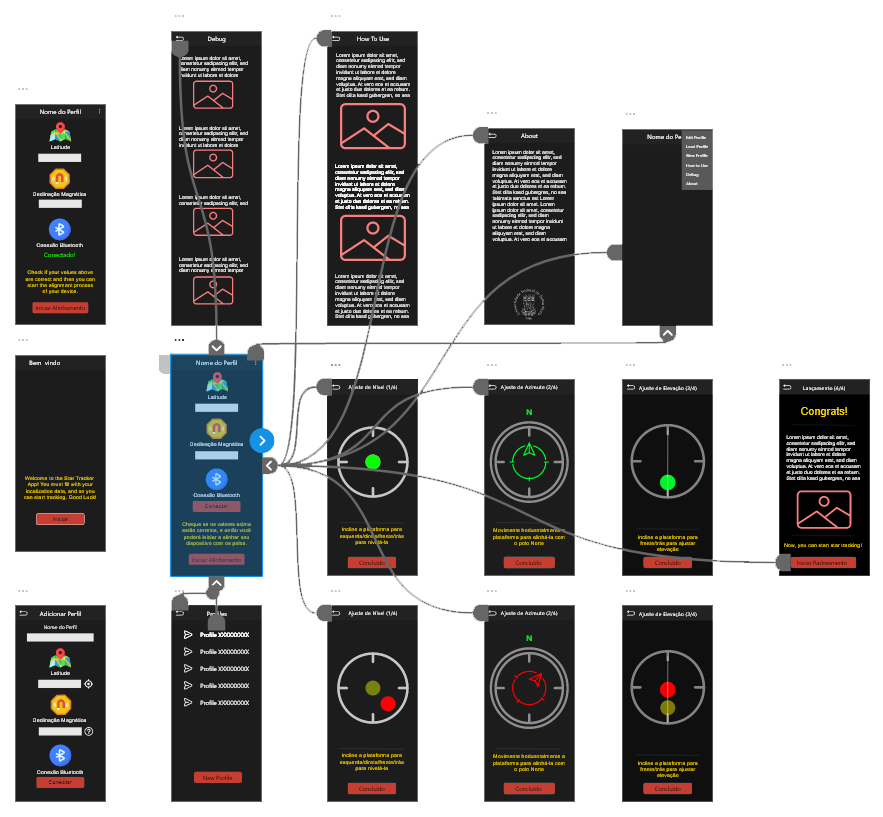
\includegraphics[width=0.7\linewidth]{figuras/desAplicativo/adobexd}
	\label{fig:adobexd}
	\fonte{Autor.}
\end{figure}

De forma geral, optou-se por usar ícones para chamar a atenção do usuário para as variáveis de posição, declinação magnética e status da conexão \textit{Bluetooth}. Como somente esses 3 dados são fundamentais para o uso da plataforma, foi possível criar um layout padrão de perfil para cada localização (Figura \ref{fig:layoutpadraoperfil}). 

\begin{figure}[!htb]
	\centering
	\caption{Esboço de tela padrão para o perfil de dados de localização}
	\includegraphics[width=0.25\linewidth]{figuras/desAplicativo/profile}
	\label{fig:layoutpadraoperfil}
	\fonte{Autor.}
\end{figure}

Além das telas de dados, o fluxo da atividade de alinhamento da plataforma foi projetado para guiar o usuário em um passo a passo simplificado. Porém, todas as telas foram desenhadas para manterem o mesmo padrão de interface, tornando a experiência mais fluída e compreensível. As demais situações foram pós implementadas diretamente durante o desenvolvimento do sistema \textit{Android}, sendo apenas abstraídas durante essa primeira etapa.

\section{Implementação do Aplicativo Android}

Diante do planejamento de interface (UI) e experiência (UX) de usuário feito anteriormente, incia-se o processo de implementação do aplicativo \textit{Android}. Três problemas precisam ser discutidos: recursos e requisitos que serão necessários para o funcionamento do aplicativo; dados a serem coletados do usuário, e; arquitetura de desenvolvimento.

\subsection{Requisitos de Sistema}

A plataforma da Google possui uma série de versões e é atualizada anualmente para os usuários finais. Porém, na realidade, o que faz um aplicativo funcionar são as inúmeras bibliotecas utilizadas durante o seu desenvolvimento, e que são atualizadas com mais frequência pela gigante de buscas. Essa realidade impõe aos desenvolvedores uma necessidade de, constantemente, se manterem atualizados e de atualizarem o código de seus aplicativos. 

Por conta dessas atualizações, existem funções de sistemas que só são disponíveis a partir de versões específicas do \textit{Android}, que é decorrente da constante evolução já mencionada. Então, por exemplo, quando um \textit{smartphone} se encontra no \textit{Android} 10, do ponto de vista do desenvolvedor isso implica que esse \textit{smartphone} trabalha com uma API \textit{Android} número 29. Consequentemente, ele terá algumas funções que não existem para o \textit{Android} 9 (API 28).

Então, ao desenvolver um aplicativo \textit{Android}, o programador deve estabelecer uma versão mínima para o qual ele irá prover suporte, e uma versão \textit{target}, que é a versão oficial em que o aplicativo operará com todos os seus recursos padrão. Normalmente, o desenvolvedor define a versão \textit{target} para ser a mais recente oferecida pela Google.

Para o caso do sistema proposto, a versão 5 do Android é a mínima para o qual é possível oferecer suporte. Isso motiva-se pois é no \textit{Android Lolipop} que a Google passa a incorporar à tecnologia \textit{Bluetooth Low Energy} no sistema. Além disso, segundo as estatísticas oferecidas pelo \textit{Android Studio}, os \textit{Smartphone} \textit{Android} com versões 5, ou superior, totalizam 98\% dos dispositivos usados no mundo\footnote{Informações obtidas no dia 1 de Fevereiro de 2022.}. 

Ou seja, oferecer suporte para \textit{smartphones} com versões inferiores à \textit{Lolipop} implica em possíveis problemas de gerenciamento de energia, relacionados a sistemas \textit{bluetooth}. Isso gera uma série de possíveis \textit{bugs} e problemas, delimitando o \textit{trade-off} entre oferecer o aplicativo para mais 2\% dos usuários ou ter de lidar com a possibilidade desses problemas. Essa definição é informada diretamente ao sistema compilador do aplicativo, \textit{Graddle}, no arquivo de construção (\textit{build}) do software, como demonstra a Figura \ref{code:compilation}  \footnote{O arquivo de \textit{build} pode ser acessado aqui: link-no-futuro}.

\begin{figure}[htb]
	\centering
	\caption{Configuração principal do compilador, no arquivo \textit{build.graddle}}
	\vspace{-15pt}
	\begin{minted}[bgcolor=codebg, fontsize=\small, frame=lines]{xml}
...
android {
	...
	defaultConfig {
		minSdkVersion 21
		targetSdkVersion 31
		...
	}
}
\end{minted}
\label{code:compilation}
\vspace{-30pt}
\fonte{Autor.}
\end{figure}

Então, a partir da definição de quais subsistemas do celular serão usados junto com o aplicativo, entende-se quais permissões são necessárias obter do usuário. Neste caso, em função da necessidade de uso do GPS e o \textit{Bluetooth}, é preciso que o usuário permita serviços de localização e comunicação. Esses serviços são definidos, com o código da Figura \ref{code:uses-permission}\footnote{O arquivo de manifesto completo pode ser acessado aqui: link-no-futuro}, no Arquivo de Manifesto - onde são declaradas todas as atividades e recursos que serão usados pelo aplicativo - e, quando forem requeridos pela aplicação, a plataforma \textit{Android} se encarregará de solicitar ao usuário a permissão, por meio de um pop-up (Figura \ref{fig:permissaoandroid}).

\begin{figure}[htb]
	\centering
	\caption{Código usado para estabelecer as permissões que serão solicitadas ao usuário.}
	\vspace{-15pt}
	\begin{minted}[bgcolor=codebg, fontsize=\small, frame=lines]{xml}
<manifest>
  <uses-permission android:name="android.permission.ACCESS_COARSE_LOCATION"/>
  <uses-permission android:name="android.permission.ACCESS_FINE_LOCATION"/>
  <uses-permission android:name="android.permission.BLUETOOTH"/>
  <uses-permission android:name="android.permission.BLUETOOTH_ADMIN"/>
  <uses-permission android:name="android.permission.BLUETOOTH_CONNECT"/>
  <uses-permission android:name="android.permission.BLUETOOTH_SCAN"/>
</manifest>
\end{minted}
\label{code:uses-permission}
	\vspace{-30pt}
\fonte{Autor.}
\end{figure}

\begin{figure}[htb]
	\centering
	\caption{Sistema Android solicitando permissão ao usuário}
	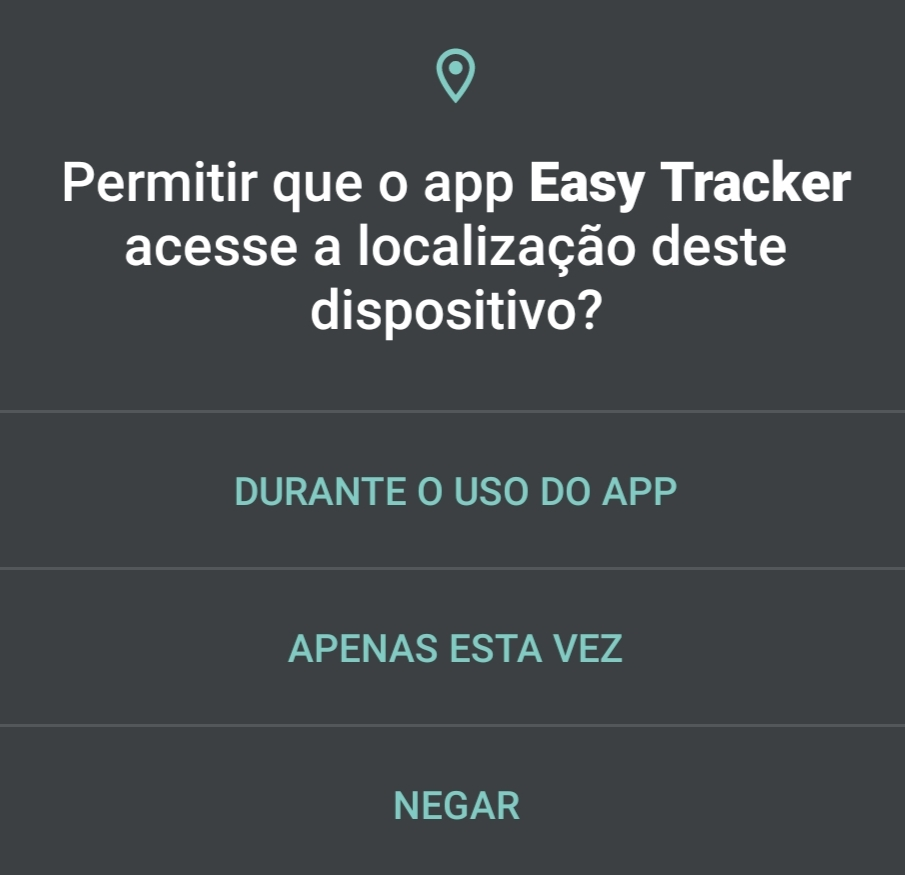
\includegraphics[width=0.35\linewidth]{figuras/desAplicativo/permission}
	\label{fig:permissaoandroid}
	\fonte{Autor.}
\end{figure}

Ademais, requisitos de espaço de armazenamento interno e memória RAM são inerentes à qualquer aplicativo. Nesse caso em específico, buscou-se simplificar ao máximo a base de dados para que o aplicativo seja o mais leve possível, também eliminando possíveis questões relacionadas a privacidade de dados do usuário.

Por isso, os únicos dados armazenados pela plataforma são aqueles que compõem a classe \textit{Profile}, que armazena os dados do perfil de localização: latitude do local, declinação magnética do local, nome do perfil e data em que as informações foram armazenadas. Além disso, uma variável que armazena o endereço MAC do dispositivo \textit{Bluetooth}, e uma \textit{flag} que indica se o perfil está sendo usado pelo usuário, também foram armazenadas. O código na Figura \ref{code:database} demonstra a criação da classe para o banco de dados\footnote{O arquivo de manifesto completo pode ser acessado aqui: link-no-futuro}.

\begin{figure}[htb]
	\centering
	\caption{Código usado para estabelecer a base de dados}
	\vspace{-15pt}
\begin{minted}[bgcolor=codebg, fontsize=\small, frame=lines]{kotlin}
@Entity(tableName = "profile_table")
data class Profile(
	@PrimaryKey(autoGenerate = true)
	var profileId: Long = 0L,
	@ColumnInfo(name = "profile_name")
	var profileName: String = "",
	@ColumnInfo(name = "last_profile")
	var lastProfile: Boolean = false,
	@ColumnInfo(name = "gps_data")
	var gpsData: String = "",
	@ColumnInfo(name = "declination")
	var declination: String = "",
	@ColumnInfo(name = "bluetooth_mac")
	var btAddress: String = "",
	@ColumnInfo(name = "start_time_milli")
	val startTimeMilli: Long = System.currentTimeMillis()
)
\end{minted}

\label{code:database}
	\vspace{-20pt}
\fonte{Autor.}
\end{figure}


\subsection{Dados e Privacidade}

Hoje em dia, a privacidade é um dos tópico muito relevante e é discutida por qualquer empresa de tecnologia. Com essa preocupação, contratos e políticas de privacidade fazem parte dessa discussão, e, por isso, é necessário que seja descrito da forma mais clara possível, para o usuário, quais e como seus dados serão usados.

Então, para o projeto, elaborou-se uma política de privacidade destacando o uso das permissões de uso de dados \textit{Bluetooth} e GPS. Os demais dados coletados não são considerados sensíveis\footnote{A política de privacidade pode ser conferida na íntegra neste link: link-no-futuro}.

\subsection{Arquitetura do Funcionamento}

A arquitetura de desenvolvimento de um aplicativo consiste na forma como a base de dados irá se comunicar com a interface de usuário, assim como buscar resolver problemas de acesso a dados em variáveis que estão sendo atualizadas em \textit{threads} concorrentes. Existem inúmeras arquiteturas consolidadas, porém a Google recomenda oficialmente o padrão \textit{Model-View-ViewModel} (MVVM) para \textit{Kotlin} e, por isso, foi usado neste software.

No MVVVM, o \textit{Model} é a parte do sistema onde as classes que representam objetos de dados são definidas. A \textit{View} consiste na atividade que está sendo mostrada na tela ao usuário, também é responsável por capturar as ações que o usuário executa ao clicar na tela. O \textit{ViewModel}, é a classe que conecta a \textit{View} com a Base de Dados, onde são declaradas as regras de negócio \cite{site:MVVM}. Nele, novas \textit{threads} são disparadas, concorrentemente, para modificar base de dados de acordo com essas regras estabelecidas pelo desenvolvedor, assim como pode se comunicar com a \textit{View}, informando quando uma alteração deve ser realizada na tela. Essa arquitetura pode ser simplificada ao diagrama da Figura \ref{fig:MVVMarc}, onde o \textit{Model} é sempre modificado por meio do \textit{ViewModel} e a \textit{View} pode disparar ações no \textit{ViewModel} quando o usuário pressiona um botão ou altera um campo de texto, por exemplo, ao passo que as modificações da \textit{View} são ordenadas pelo \textit{ViewModel}, por meio das regras de negócio.

\begin{figure}[htb]
	\centering
	\caption{Arquitetura MVVM genérica.}
	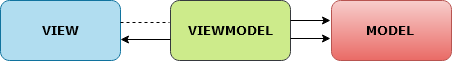
\includegraphics[width=0.45\linewidth]{figuras/desAplicativo/MVVMarc}
	\label{fig:MVVMarc}
	\fonte{\cite{site:MVVM}.}
\end{figure}


No desenvolvimento \textit{Android}, em \textit{Kotlin}, o \textit{Model} é normalmente uma Base de Dados \textit{ROOM}, que é o nome da biblioteca que permite criar e manipular Bancos de Dados com \textit{querys} SQL. O \textit{ViewModel} é uma classe específica que coordena as \textit{Views} com regras de negócio. As \textit{Views} são declaradas como \textit{Activity} ou \textit{Fragments} \cite{site:MVVM}. A aplicação da arquitetura MVVM dentro do ambiente android é descrita na Figura \ref{fig:MVVM}, considerando também o uso de APIs remotas - \textit{Webservices} - para obter acesso a dados, que pode ser realizado com a biblioteca \textit{Retrofit}, mas que não foi utilizado neste trabalho. 

\begin{figure}[htb]
	\centering
	\caption{Arquitetura MVVM aplicada ao sistema \textit{Android}, em \textit{Kotlin}}
	\includegraphics[width=0.45\linewidth]{figuras/desAplicativo/MVVM}
	\label{fig:MVVM}
	\fonte{Adaptado de \cite{site:MVVM}.}
\end{figure}
% https://digital-solutions.consulting/blog/mvvm-and-its-implementation-in-android/

A \textit{Activity} consiste na Atividade que está sendo executada. Um aplicativo pode possuir várias atividades internamente, que se conectam de acordo com regras de interface, exemplo: um usuário acessa uma atividade restrita a telas de login, onde ele faz um cadastro ou preenche suas informações de login; quando ele realiza o login, uma nova atividade é iniciada com as próximas telas do aplicativo carregadas. O \textit{Fragment} consiste em cada tela exibida dentro de uma \textit{Activity}. No exemplo anterior, a \textit{Activity} de \textit{login} pode conter um \textit{Fragment} para o cadastro inicial e outro \textit{Fragment} para o usuário inserir suas credenciais (e-mail e senha) de acesso à aplicação (Figura \ref{fig:exemploActivity}). 


\begin{figure}[!htb]
	\centering
	\caption{\textit{Fragments} dentro de uma mesma \textit{Activity}}
	\includegraphics[width=0.3\linewidth]{figuras/desAplicativo/exemploActivity}
	\label{fig:exemploActivity}
	\fonte{Autor.}
\end{figure}

O \textit{ViewModel} se conecta com a \textit{View} por meio de \textit{databinding}. Com ele, é possível conectar um dado que é mostrado na \textit{View} diretamente ao \textit{ViewModel}, assim como conectar funções executadas no pressionar de um botão. Isso é possível com a Classe de dados \textit{MutableLiveData}, que diferencia-se de outras variáveis pois é possível disparar funções somente quando ela é alterada. Com isso, o sistema não precisa monitorar a todo instante quando um dado é editado, de maneira automática e economizando processamento. 

A \textit{View} é construída em um arquivo XML, onde é definido o \textit{layout} e como os componentes se comportarão na tela do usuário. Neste arquivo, a instância de dados -- que irá se comunicar por \textit{databinding} -- é criada, referenciando-a ao \textit{ViewModel}, como demonstra o código da Figura \ref{code:layoutdata}.
 Dessa maneira, é possível conectar um texto diretamente à uma variável da regra de negócios, ou também conectar um botão à uma função (Figura \ref{code:viewmodelbutton}). Essas variáveis e funções são declaradas dentro da classe de \textit{ViewModel} referente ao \textit{fragment} onde está sendo referenciada, simplificado na Figura \ref{code:viewmodel}.

\begin{figure}[!htb]
	\centering
	\caption{Declaração do \textit{ViewModel} dentro do \textit{layout}, no \textit{Fragment} que cria um novo perfil de localização}
	\vspace{-15pt}
	\begin{minted}[bgcolor=codebg, fontsize=\small, frame=lines]{xml}
<layout>
	...
	<!-- Disponibiliza os dados do ViewModel para realizar databinding. -->
	<data>
	<variable
	name="newProfileViewModel"
	type="com.epp.easytracker.newprofile.NewProfileViewModel" />
	</data>		
</layout>
	\end{minted}
	\label{code:layoutdata}
	\vspace{-30pt}
	\fonte{Autor.}
\end{figure}

\begin{figure}[!htb]
	\centering
	\caption{Código dentro do \textit{layout} de um \textit{fragment} para conectar um texto à uma variável, e um botão à uma função que aciona o \textit{ViewModel} diretamente}
	\vspace{-15pt}
	\begin{minted}[bgcolor=codebg, fontsize=\small, frame=lines]{xml}
<layout>
	...
	<!-- Campo de declinação magnética. 
		Quando o usuário editar, 
		esse dado irá direto para o ViewModel -->
	<com.google.android.material.textfield.TextInputEditText
	android:inputType="numberDecimal"
	android:text="@={newProfileViewModel.magDeclination}"
	android:textSize="18sp"
	/>
	
	<!-- Quando o botão for pressionado, 
		o ViewModel será sinalizado -->
	<Button
	android:id="@+id/button_connect"
	android:onClick="@{() -> newProfileViewModel.onStartConnection()}"
	/>
	...
</layout>
	\end{minted}
	\label{code:viewmodelbutton}
	\vspace{-30pt}
	\fonte{Autor.}
\end{figure}


\begin{figure}[!htb]
	\centering
	\caption{Código do \textit{ViewModel}, que se conectará com a \textit{View} por \textit{Databinding}}
	\vspace{-15pt}
	\begin{minted}[bgcolor=codebg, fontsize=\small, frame=lines]{kotlin}
package com.epp.easytracker.newprofile

//declaração do viewModel
class NewProfileViewModel(
	val database: ProfileDatabaseDao,
	application: Application
) : AndroidViewModel(application) {		
	...
	// variável mutável para ser acessada por databinding
	var magDeclination = MutableLiveData<String>()
	
	// função pública para ser acessada via databiding
	// informa ao viewmodel que o botão de
	// conexão bluetooth foi pressionado
	fun onStartConnection(){
		viewModelScope.launch {
			_startConnection.value = true
		}
	}
	...
}
	\end{minted}
	\label{code:viewmodel}
	\vspace{-30pt}
	\fonte{Autor.}
\end{figure}

\subsection{Protocolo de Comunicação \textit{Bluetooth}}

Dentro dos componentes de arquitetura, o \textit{Bluetooth} se encontra fora de qualquer estrutura. Ele funciona com \textit{threads} separadas, mas sua classe é necessariamente atrelada à uma \textit{Activity} e ao contexto de um \textit{Fragment}. Entre outras palavras, o \textit{Bluetooth} do celular só se comunica com o aplicativo se estiver associado aos elementos da tela. Por esse motivo, estabeleceu-se que toda a seção principal, de perfil de localização e alinhamento, consistiria em uma atividade única. Caso o aplicativo fosse dividido em mais \textit{Activitys}, o sistema necessariamente iria desconectar o \textit{Bluetooth} quando elas fossem alternadas. Em termos práticos, o \textit{Bluetooth} iria reconectar com a eletrônica em cada alternância de telas, criando uma preocupação indesejada para o usuário. 

A conexão é realizada usando o endereço MAC do dispositivo com que deseja-se comunicar. Para a comunicação iniciar, indica-se ao sistema, qual o serviço \textit{Bluetooth} adotado pela eletrônica, ou seja, seu UUID. Para o caso do chip HC-05 empregado, o código como o da Figura \ref{code:bluetoothconnection} realiza a conexão.

\begin{figure}[!htb]
	\centering
	\caption{Código simplificado para estabelecer a base de dados}
	\vspace{-15pt}
	\begin{minted}[bgcolor=codebg, fontsize=\small, frame=lines]{kotlin}
...
private lateinit var mmDevice: BluetoothDevice // dispositivo
private lateinit var mmInStream: InputStream // buffer de entrada
private lateinit var mmOutStream: OutputStream // buffer de saída
private lateinit var mmAdapter: BluetoothAdapter 
lateinit var mmSocket: BluetoothSocket
private val myUUID: UUID? =
	UUID.fromString("00001101-0000-1000-8000-00805F9B34FB")
fun connectThread(context: Context) {
	val bluetoothManager =
		context.getSystemService(Context.BLUETOOTH_SERVICE)
		as BluetoothManager
	
	// checa se o dispositivo suporta comunicação Bluetooth
	// e se ela está ativada
	if (bluetoothManager.adapter != null) {
		mmAdapter = bluetoothManager.adapter
		if (!mmAdapter.isEnabled) {
			throw Exception(
				"Bluetooth adapter não encontrado ou acionado!")
		}
		...
		// Declara o dispositivo pelo seu endereço MAC
		mmDevice = mmAdapter.getRemoteDevice(DeviceMAC)
		// Realiza a Conexão
		mmSocket = mmDevice.createRfcommSocketToServiceRecord(myUUID)
		...
		try {
			mmSocket.connect()
			// Aciona os Buffers I/O de dados bluetooth
			mmInStream = mmSocket.inputStream
			mmOutStream = mmSocket.outputStream
			
		} catch (e: IOException) {
			...
		}
	}
	...
}		
	\end{minted}
	\label{code:bluetoothconnection}
	\vspace{-30pt}
	\fonte{Autor.}
\end{figure}

Para este trabalho, a comunicação do \textit{smartphone} com a plataforma equatorial é sempre iniciada pelo celular. O aplicativo envia mensagens de confirmação da comunicação em uma taxa de 2Hz. Com isso, a eletrônica sabe que pode enviar mensagens para o aplicativo e quais informações enviar. Caso o aplicativo não envie mensagens ou não haja conexão, a eletrônica não permanece utilizando sistema \textit{Bluetooth} e assim economiza energia. 

A comunicação estabelecida como padrão ocorre no cenário de alinhamento, onde o aplicativo envia o \textit{char} '0' como confirmação da comunicação, e a plataforma transmite os dados dos ângulos inerciais. Quando é preciso alterar o estado da eletrônica para que inicie a calibração ou rastreamento, outro \textit{char} é enviado. Então a plataforma envia ao celular uma mensagem com dois \textit{char}, confirmando a alteração de estado. Isso é realizado da seguinte forma, para cada cenário:

\begin{itemize}
	\item Iniciar rastreamento: \textit{smartphone} envia o \textit{char} 's', plataforma envia string "s,s$ \backslash $n"
	\item Parar o rastreamento: \textit{smartphone} envia o \textit{char} 'n', plataforma envia string "n,n$ \backslash $n"
	\item Calibrar a bússola: \textit{smartphone} envia o \textit{char} 'c', plataforma envia string "c,c$ \backslash $n"
\end{itemize}

Ao receber essas strings, o aplicativo altera \textit{flags} dentro da classe \textit{bluetooth}. Essas variáveis são declaradas como \textit{MutableLiveData} e indicam diretamente à \textit{View} quando houve uma alteração na plataforma, confirmando ao usuário que foi iniciado o rastreamento ou a calibração. Quando o \textit{smartphone} envia o valor '0' e a plataforma não está em estado de rastreamento ou calibração, a comunicação segue o padrão. 

Os dados recebidos na comunicação passam por um \textit{buffer} de 230 \textit{bytes}, e o aplicativo tem acesso aos dados armazenados nele após ter sido inteiramente preenchido ou se houver passado o \textit{timeout} do sistema Android. O tempo para a eletrônica enviar 230 \textit{bytes}, somado a latência do \textit{Bluetooth}, implicam no tempo total de intervalo (\textit{delay}) entre as informações serem captadas pelos sensores e aparecerem na tela para usuário. Como as mensagens são enviadas pela plataforma em 9600 bits por segundo, existe uma defasagem de, pelo menos, $ 230\times8/9600 = 192 $ milissegundos.  

Assim, constata-se que, quanto mais rápido o sistema for capaz de enviar as informações, mais rápido o \textit{buffer} será preenchido. Se o \textit{buffer} não é preenchido, observou-se que o \textit{Android} libera os dados após um período limite (\textit{timeout}). Além disso, outro fator relevante é o tamanho do pacote. Quanto menor for o pacote de dados contendo os ângulos inerciais do \textit{EasyTracker}, mais atualizações de tela serão possíveis no aplicativo, promovendo maior fluidez da interface. 

Quando o usuário está em processo de alinhamento, e solicita dados dos ângulos para a plataforma, a Eletrônica é responsável por realizar todos os cálculos com os dados do IMU e enviar para o \textit{smartphone} os três ângulos inerciais juntamente com uma chave de validação. Esses 4 valores são enviados entre vírgulas, e com uma quebra de linha no final da mensagem, com o caracter "$\backslash$n", como demonstra a representação na Figura \ref{fig:pacoteBT}. Além disso, para compactar a mensagem, os valores em ponto flutuante que armazenam os ângulos na eletrônica são convertidos para um valor inteiro. Para não perder precisão, o valor é multiplicado por 10 antes de ser convertido. Com isso, o tamanho do pacote passa a ser de $ 2+1+2+1+2+1+2+1 = 12 $ \textit{bytes}. Logo, resta ao aplicativo: extrair, validar e mostrar os dados do \textit{buffer} ao usuário.

\begin{figure}[!htb]
	\centering
	\caption{Pacote de dados transmitido no cenário de alinhamento}
	\includegraphics[width=0.6\linewidth]{figuras/desAplicativo/pacoteBT}
	\label{fig:pacoteBT}
	\fonte{Autor.}
\end{figure}

A extração dos dados é feita por meio da vírgula e do caracter de final de linha. Com o fim de linha separam-se os pacotes dentro do \textit{buffer}, e os valores dentro de cada pacote são separados com o caractere de vírgula. A validação mencionada é necessária pois a comunicação \textit{bluetooth} não garante a integridade dos dados enviados na mensagem, que são interpretados como uma \textit{String}. Isso é realizado de duas formas: conferindo se a estrutura da \textit{String} de dados está correta, e se os valores estão corretos. 

A verificação da estrutura é realizada comparando se a quantidade de valores recebidos é de 4 elementos; na sequência, a verificação de dados é feita com o quarto dado do vetor, que é calculado na eletrônica como a soma dos 3 primeiros valores. No aplicativo é feito o mesmo processo: somam-se os 3 primeiros valores e essa soma é comparada com o quarto valor enviado pela eletrônica. Se o dado calculado for igual à chave, significa que os dados mantiveram sua integridade e podem ser mostrados ao usuário. Caso contrário, são descartados. Esse processamento é descrito no diagrama da Figura \ref{fig:validacaobluetooth}.

\begin{figure}[!htb]
	\centering
	\caption{Diagrama de processamento empregado no lado do Aplicativo}
	\includegraphics[width=\linewidth]{figuras/desAplicativo/validacaobluetooth}
	\label{fig:validacaobluetooth}
	\fonte{Autor.}
\end{figure}

Todos esses dados são processados dentro da classe \textit{Android} de Serviço \textit{Bluetooth}, onde são declaradas duas \textit{flags}, uma indicando o status da comunicação, e outra indicando se um novo dado foi processado. A comunicação dessa \textit{thread} com os \textit{fragments} é realizado utilizando a classe \textit{MutableLiveData} para monitorar as \textit{flags}, similar ao processo de \textit{databinding}. Assim, é possível atualizar os itens mostrados na tela, ou também determinar quando um erro de comunicação ocorreu por falha de conexão. 

No caso de erro de comunicação, o aplicativo chama a atenção do usuário por meio do \textit{popup} na Figura \ref{fig:popupreconect}, informando que não está mais conectado e questionando se o usuário deseja se reconectar. Assim, novamente, processamento é economizado, pois a interface irá atualizar somente quando houver mudanças no status da comunicação, ou se existirem novos dados a serem recebidos.

\begin{figure}[!htb]
	\centering
	\caption{\textit{Popup} padrão para reconectar com a Eletrônica}
	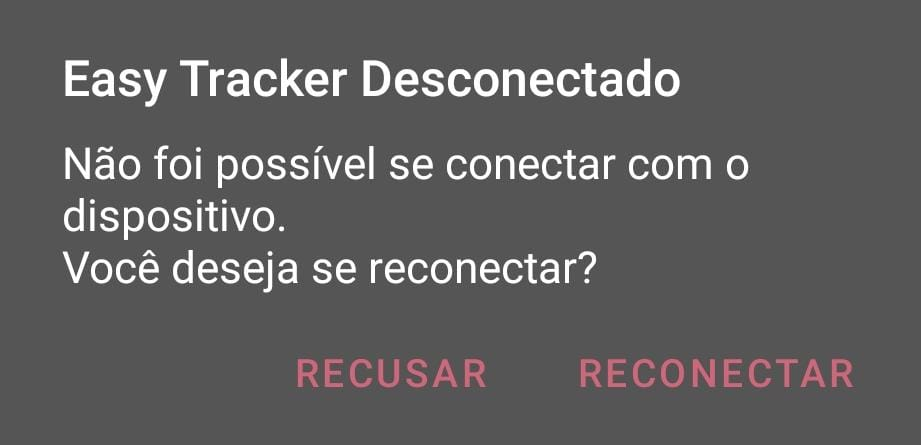
\includegraphics[width=0.4\linewidth]{figuras/desAplicativo/popupreconect}
	\label{fig:popupreconect}
	\fonte{Autor.}
\end{figure}

Portanto, a arquitetura final do sistema pode ser demonstrada na Figura \ref{fig:finalarc}. A estrutura de comunicação \textit{Bluetooth} possui suas próprias regras de negócio e se comunica direto com a \textit{View} para modificar as informações mostradas ao usuário. O \textit{ViewModel} controla apenas as demais regras, englobando navegação entre os \textit{Fragments} e base de dados

\begin{figure}[!htb]
	\centering
	\caption{Arquitetura final do aplicativo}
	\includegraphics[width=0.6\linewidth]{figuras/desAplicativo/finalarc}
	\label{fig:finalarc}
	\fonte{Autor.}
\end{figure}